This chapter presents a detailed explanation of the neural network models proposed in this work and
the correspondent baselines used for comparison. In Section \ref{sec:problem_def} we give a formal definition
of the learning problem. In Section \ref{sec:nn_arch} the architectures of
the main networks are shown. In Section \ref{sec:adds} we detailed additional components used on the models and training.
Finally, Section \ref{sec:baselines} shows the baselines models
used for the ablation study of both performance and explainability.


\section{Problem Definition}
\label{sec:problem_def}

Following a formulation similar to \citeA{hidalgo_placepulse}, each attribute $A$ in the PP 2.0
consists of a set $I_A$ of images and a set $P_A$ of votes for those images.
Each image in $I_A$ is a tensor $x \in \mathbb{R}^{h \times w \times 3}$ where $h$ and $w$ are the height and width respectively.
Each vote in $P_A$ is a triple $(x_1,x_2,y)$ where $x_1$ and $zx_2$ are images in $I_A$ and $y\in \{1,0,-1\}$.
A triple $(x_1,x_2,y)\in P_A$ represents a comparison where $y=1$ states a preference of $x_1$ over $x_2$, and $y=-1$
represents a preference of $x_2$ over $x_1$. The value $y=0$ represents a tie.

The objective is to, for each attribute, learn a ranking function $f_A : \mathbb{R}^{h \times w \times 3} \rightarrow \mathbb{R}$
that maps the image tensor to an urban perception score, satisfying the order given by the votes. Formally the
maximum amount of the following constraints need to be satisfied:

\begin{equation}
	y \cdot (f_A(x_1) - f_A(x_2)) > 0 \;  \forall (x_1,x_2,y) \in P_A\text{ and }y\in\{-1,1\}
	\label{eq:constraints}
\end{equation}

Unlike the previous literature, tie votes are also used in this work, generating the following additional constraints:

\begin{equation}
	|f_A(x_1) - f_A(x_2)| < m \;\; \forall (x_1,x_2,y) \in P_A\text{ and }y=0 \; ;  m \in \mathbb{R}^+
	\label{eq:constraints_ties}
\end{equation}

Where $m$ is a constant margin.

Since $f_A$ is intended to learn a ranking of the input images, it is desirable that the function defines an order
on the image space so that the ranking results are consistent. This condition can and should be enforced by
model design \cite{koppel_pairwise}, but since the data is crowdsourced without
validation, the constraints generated by equation \ref{eq:constraints}, do not represent a  100\% transitive order.
Because of that, it is infeasible for a model designed for ranking and therefore
transitive by construction, to satisfy all of them.
This issue makes it harder to obtain high scores in accuracy based metrics in practice, and
those are the only ones available in the literature so far.


\section{Network architectures}
\label{sec:nn_arch}
As was mentioned before, the main principle followed for model design is to enhance explainability
while maintaining performance of the model as much as possible. With that in mind, we combine two
state-of-the-art techniques from the deep learning literature, semantic segmentation
and attention mechanisms, to design three novel architectures that present a significant
improvement in explainability over traditional blackbox CNNs. We describe these architectures
in the following sub sections, ordered by model complexity. Is important to note that
for learning to rank on the PlacePulse dataset,
two forward passes of the ranking  network are required for each data instance (one for each image) and both scores are used
for calculation of the loss. See section \ref{section:loss} for  details.


\subsection{SegRank base.}
The traditional deep learning approach in computer vision, consists of using a pretrained
CNN \cite{lecun_mnist}, on the Imagenet dataset \cite{imagenet}, such as the ResNet \cite{he_resnet},
usually called the feature extractor, and then stacking a custom set of layers over its output features. Leaving the CNN weights
fixed or updating them on training  depends on the particular problem. This is the approach taken
by most of the previous literature on urban perception \cite{hidalgo_placepulse,tamara_judgments,zhang_measuring}.

In this work, we propose replacing the traditional feature extractors for a fully trained semantic segmentation
network. The semantic segmentation task consists of assigning a label to every pixel in an image, and therefore
it implies a fine grained detection of object edges, providing a rich amount of information that is human understandable.
The output of a semantic segmentation model is a probability distribution over the different classes for each pixel,
making it usable as a feature map of the image. See Figure \ref{fig:segmentation} for an example.

We base our models on the PSPNet architecture \cite{pspnet}, since it is one of the highest performing models
available in the literature. It's design is based on a ResNet50 and a pyramid pooling module, which consists on
parallel poolings and convolutions at different scales, that are then concatenated and used to generate the output with a
final convolution.

\begin{figure}[ht]
	\begin{center}
	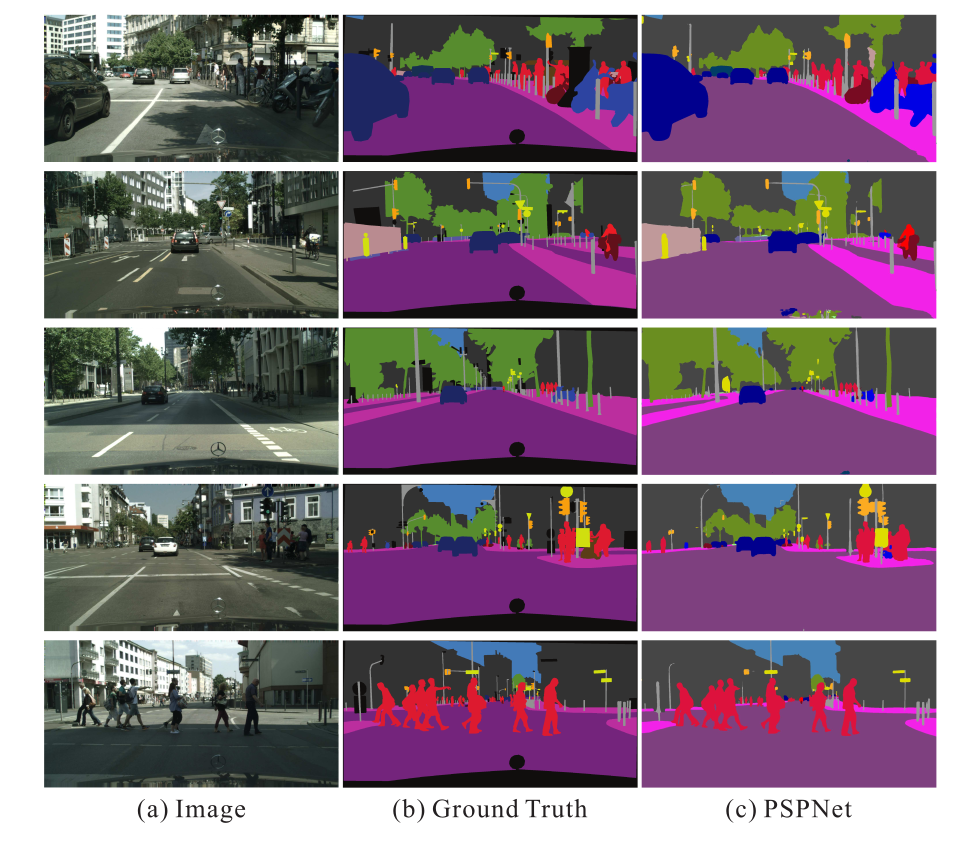
\includegraphics[width=0.8\textwidth]{./figures/segmentation.png}
	\caption[Example of Semantic Segmentation]{Examples of semantic segmentation by the PSPNet model on the CityScapes dataset. Extracted from \citeA{pspnet} }
	\label{fig:segmentation}
	\end{center}
\end{figure}

\begin{figure}[ht]
	\begin{center}
	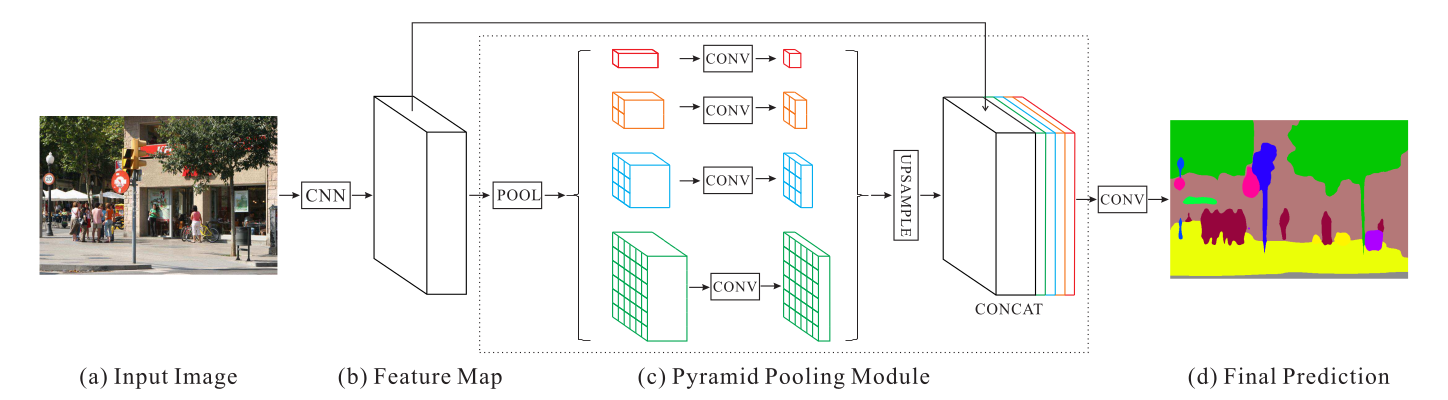
\includegraphics[width=0.9\textwidth]{./figures/pspnet.png}
	\caption[PSPNet architecture]{PSPNet architecture. Extracted from \citeA{pspnet} }
	\label{fig:segmentation}
	\end{center}
\end{figure}

We train PSPNet on the CityScapes dataset \cite{cordts_cityscapes}, since its urban images taken from a car have
considerable similarity to Street View images, and its classes have proven informative for the urban perception problem
in previous research \cite{rossetti,zhang_measuring}. After this process we keep the network weights fixed
and use the output as features for subsequent layers. The segmentation output  is a tensor $S$, $S \in \mathbb{R}^{h\times w \times C}$, with $C$
being the number of different classes. We experiment with using the features directly or applying a softmax operation.

For the calculation of the ranking score, we apply a linear transformation to every pixel distribution, flattening the output to
$\mathbb{R}^{h \times w}$  and then an MLP with one hidden layer and ReLU activation. The final linear layer
of the MLP generates a single scalar value representing the perception score.

It is important to note that the features given by  segmentation are  of considerable less dimensionality
than traditional ResNet features and only capture the very specific information of which class is each pixel,
which makes them  significantly less expressive. Adding to that,
since traditional CNN based approaches allow for finetuning, the amount of trainable parameters
is also much smaller for this model than traditional models. Due to these two reasons the learning capacity
of this model is much smaller, and therefore a significant performance drop is likely to happen.

\begin{figure}[ht]
	\begin{center}
	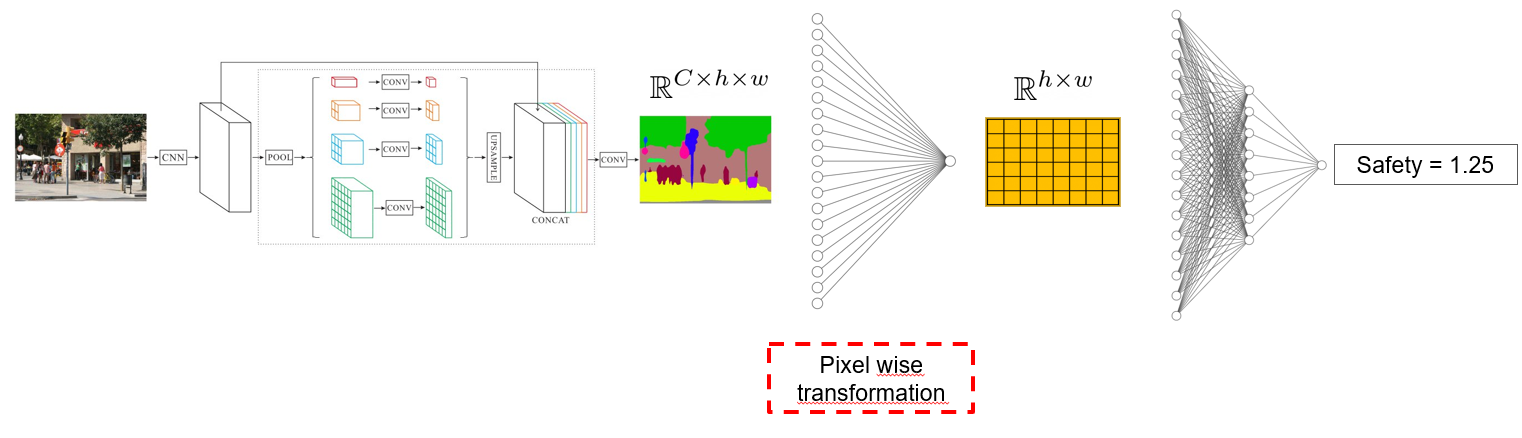
\includegraphics[width=0.9\textwidth]{./figures/segrank_1.png}
	\caption[First model architecture]{First model architecture}
	\label{fig:segrank_1}
	\end{center}
\end{figure}

\subsection{SelfSegRank}\label{section:self-attn}
With the intention of improving  performance and explainability of SegRankBase model, we process
the segmentation output with self attention mechanisms instead of a traditional MLP,
since it has been proven to provide benefits in both aspects by previous research \cite{vaswani_attention, wiegreffe_attention, cordonnier_relationship}.

For our model we use the scaled dot product attention mechanism
proposed by \citeA{vaswani_attention}. We abstain from using the full multi head attention
mechanism  that consists of the same operations but splitting the input in several ``heads''.
We do this because using multiple heads adds complexity to the interpretation of the attention outputs,
since different heads may output inconsistent weights, as is mentioned in \citeA{clark_bertlook}
and \citeA{li_disagreement} and also verified on this task by our own experiments.

The attention mechanisms receives three matrixes as input: the query $Q$, the key $K$ and the value
$V$. It calculates a matrix of attention weights over $V$ based on $Q$ and $K$ and the final output
is given by the product between $V$ and the weights. A linear transformation is defined
for each of the inputs with weights $W_Q, W_K, W_V$ respectively, and another transformation $W$
is applied to the final output (see Figure \ref{fig:attention_mech}).
Formally the attention layer can be defined as:
\begin{align}
	\label{eq:attention}
	\text{Attention}(Q,K,V) &= \text{softmax}\left (\frac{QK^T}{\sqrt{d_k}} \right ) V \\
	\label{eq:attention_layer}
	\text{AttentionLayer}(Q,K,V) &=  \text{Attention}(QW_Q,KW_K,VW_V)\cdot W
\end{align}
where $d_k$ is the embedding size of the key. For the particular case of self attention,
the same input is used as query, key and value, so for our case we make $Q=K=V=S'$ with
$S' \in \mathbb{R}^{(hw) \times C}$ and equal to the segmentation output flattened to one
spatial dimension.

\begin{figure}[ht]
	\begin{center}
	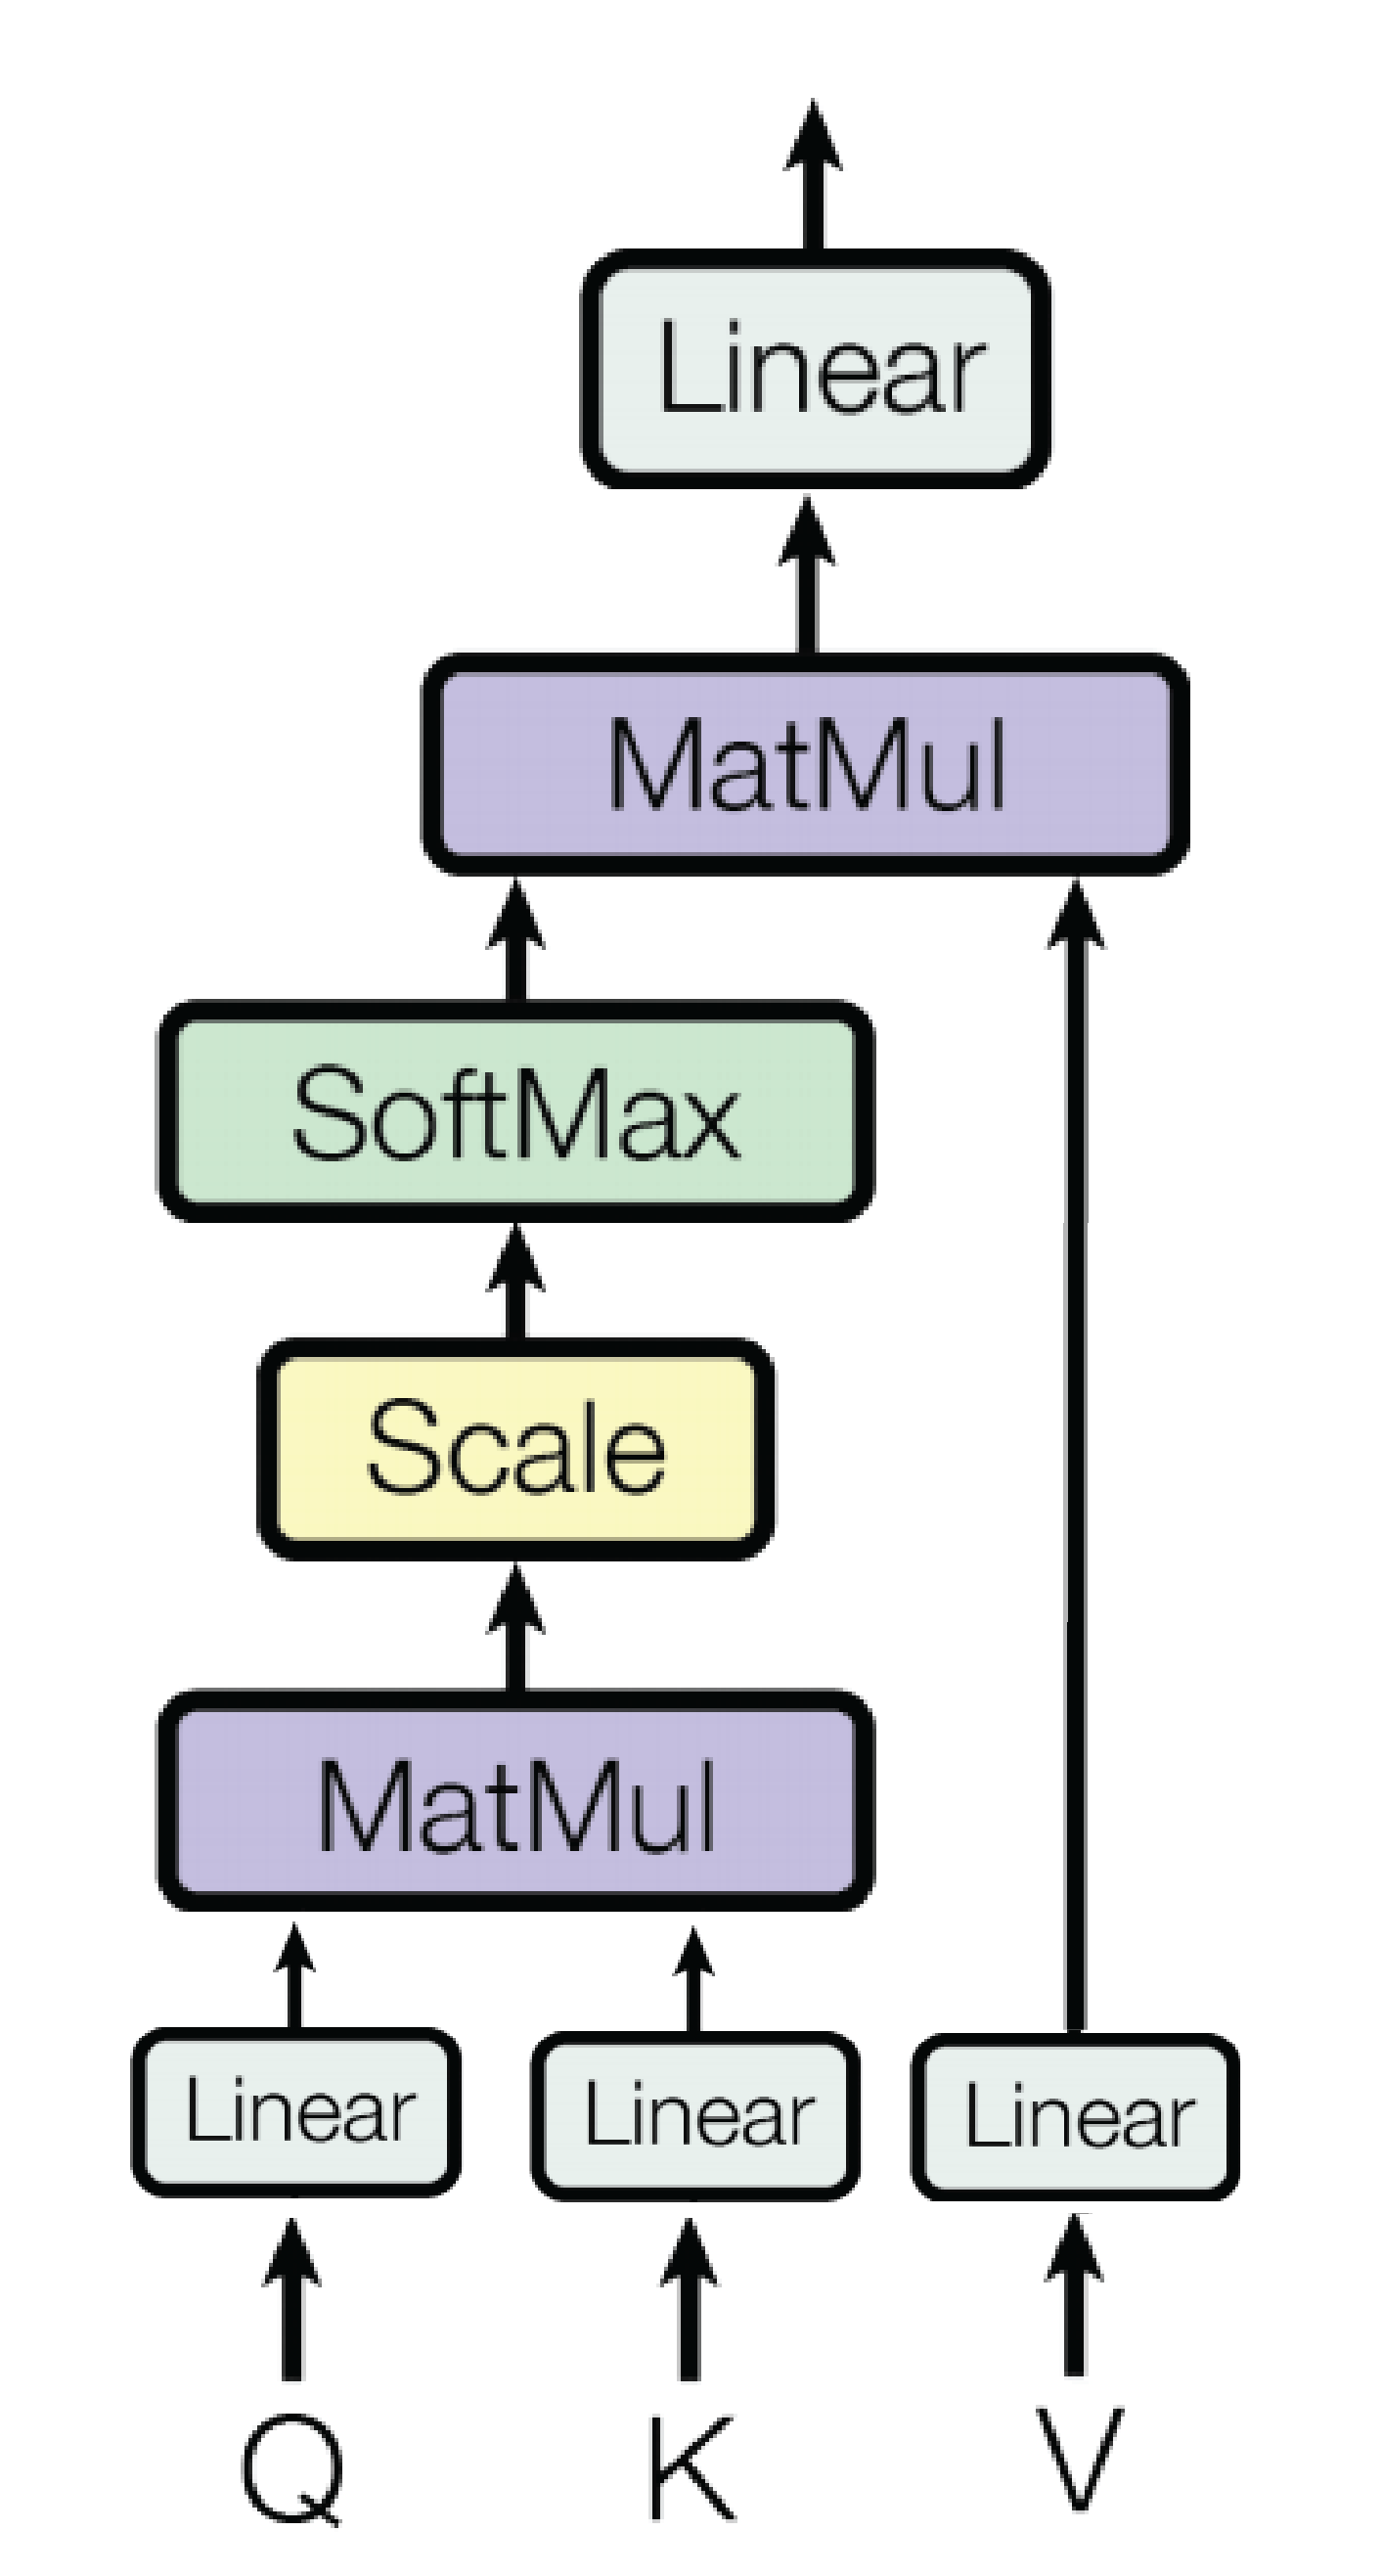
\includegraphics[width=0.3\textwidth]{./figures/attention.png}
	\caption[Attention Mechanism]{Attention layer operations. Adapted from \citeA{vaswani_attention}}
	\label{fig:attention_mech}
	\end{center}
\end{figure}

Similarly to the previous model, we apply a linear layer to calculate the ranking score from the attention output.
We only use one layer instead of two in this model because the attention mechanism already has a large amount of parameters and a
linear transformation of its own.
In parallel the attention weights are also outputted by the model and are used for visualization. Figure \ref{fig:selfsegrank}
shows a diagram of the full architecture

\begin{figure}[ht]
	\begin{center}
	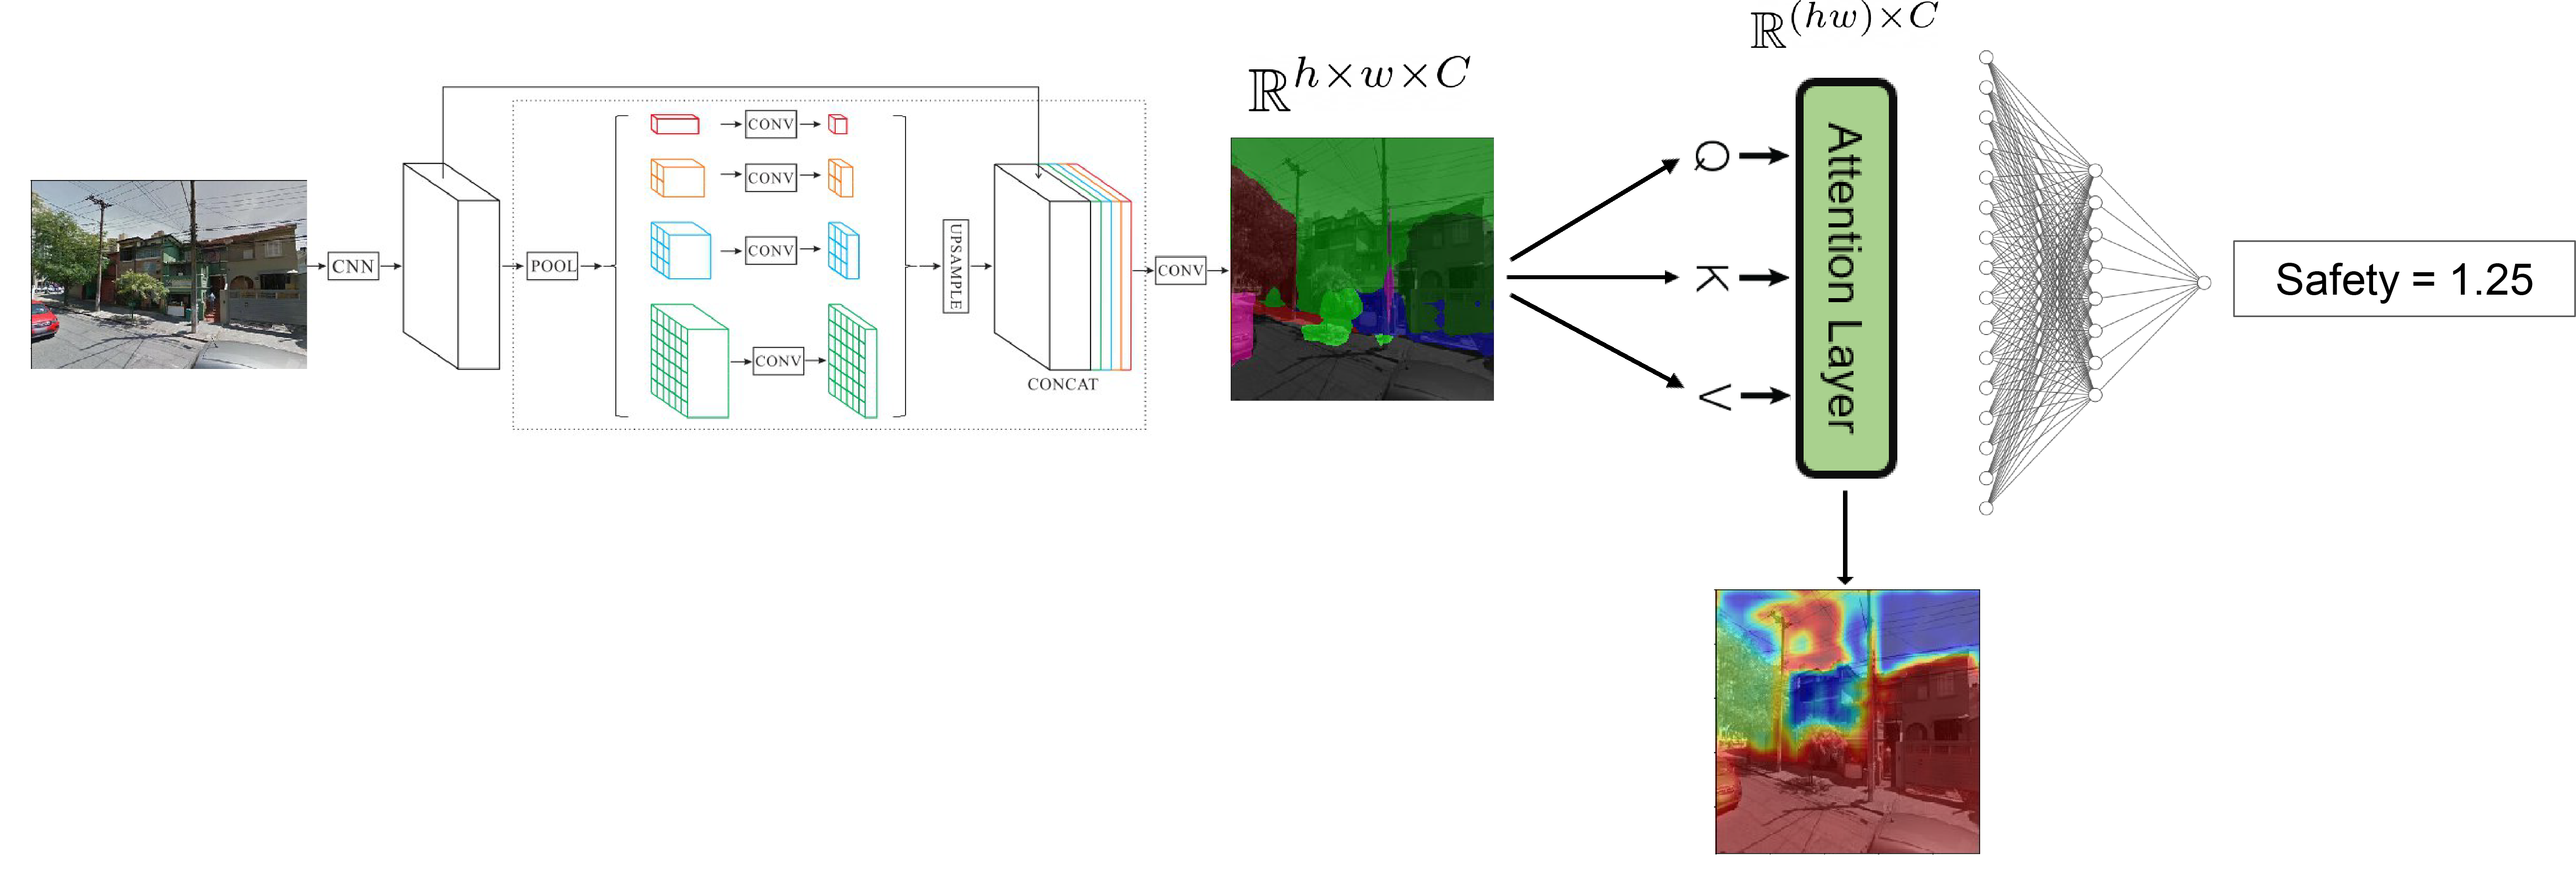
\includegraphics[width=1\textwidth]{./figures/self_attn.png}
	\caption[Self Attention network]{Segmentation and self attention network.}
	\label{fig:selfsegrank}
	\end{center}
\end{figure}

\begin{figure}[ht]
	\begin{center}
	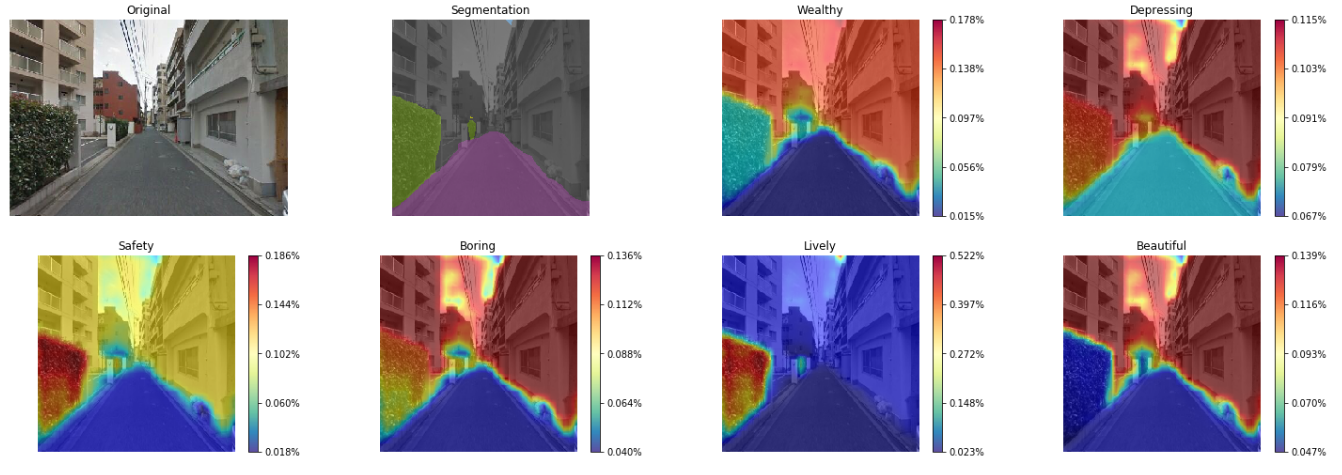
\includegraphics[width=1\textwidth]{./figures/self_attn_vis.png}
	\caption[Self Attention Model output]{Example segmentation and self attention weights for all six attributes.}
	\label{fig:segrank_attention}
	\end{center}
\end{figure}

As it can be seen on Figure \ref{fig:segrank_attention}, the attention weights keep the object shapes,
allowing for a clear interpretation of which objects are significant to the output.

\subsection{AttentionSegRank}
As was mentioned before, segmentation based features are considerably less expressive than
traditional deep CNN features and cannot be finetuned, generating an important trade off between explainability and model performance.
As a solution to that problem, we propose a mixed approach, that weights in both the image segmentation
and the CNN features, in order to achieve both good performance and interpretability. To do that,
we take advantage of the multiple inputs in the scaled dot product attention mechanism. The method consists
of using the segmentation as key, and the ResNet features as both query and value (see equations \ref{eq:attention} and \ref{eq:attention_layer} ).

In practice, $K$ and $V$ must have the same spatial dimension for equation \ref{eq:attention} to be valid.
We solve this problem by using layer \textit{conv\_4f} of ResNet50 instead of \textit{conv\_5c}  , since it has a
larger spatial dimensionality, and we add a transposed convolution layer \cite{noh_deconv} to do the final upsampling
required to match the segmentation output dimension.

We do this because using the segmentation as key induces the attention weights to maintain a similar shape as the segmentation objects,
keeping interpretability. To understand why this happens, see the $QK^t$ product on equation \ref{eq:attention} that generates the
weight matrix. A single element of the matrix (or a single attention weight) is given by:
\begin{align}
	a_{ij} = \sum_{l=1}^d q_{il}k_{jl}
\end{align}

With $a_{ij}$ being the weight that the value feature $v_j$ has on output feature $i$. Setting up $K=S'$  and $Q=F'$, with $S'$ and $F'$ the flattened segmentation and ResNet features
respectively:
\begin{align}
	a_{ij} = \sum_{l=1}^d f_{il}s_{jl}
\end{align}

Meaning that the weight of feature $j$ on output feature $i$ depends on which object is pixel $j$, resulting in an attention weight matrix
that keeps the  interpretability of the segmentation objects independently of the convolutional features.

\begin{figure}[ht]
	\begin{center}
	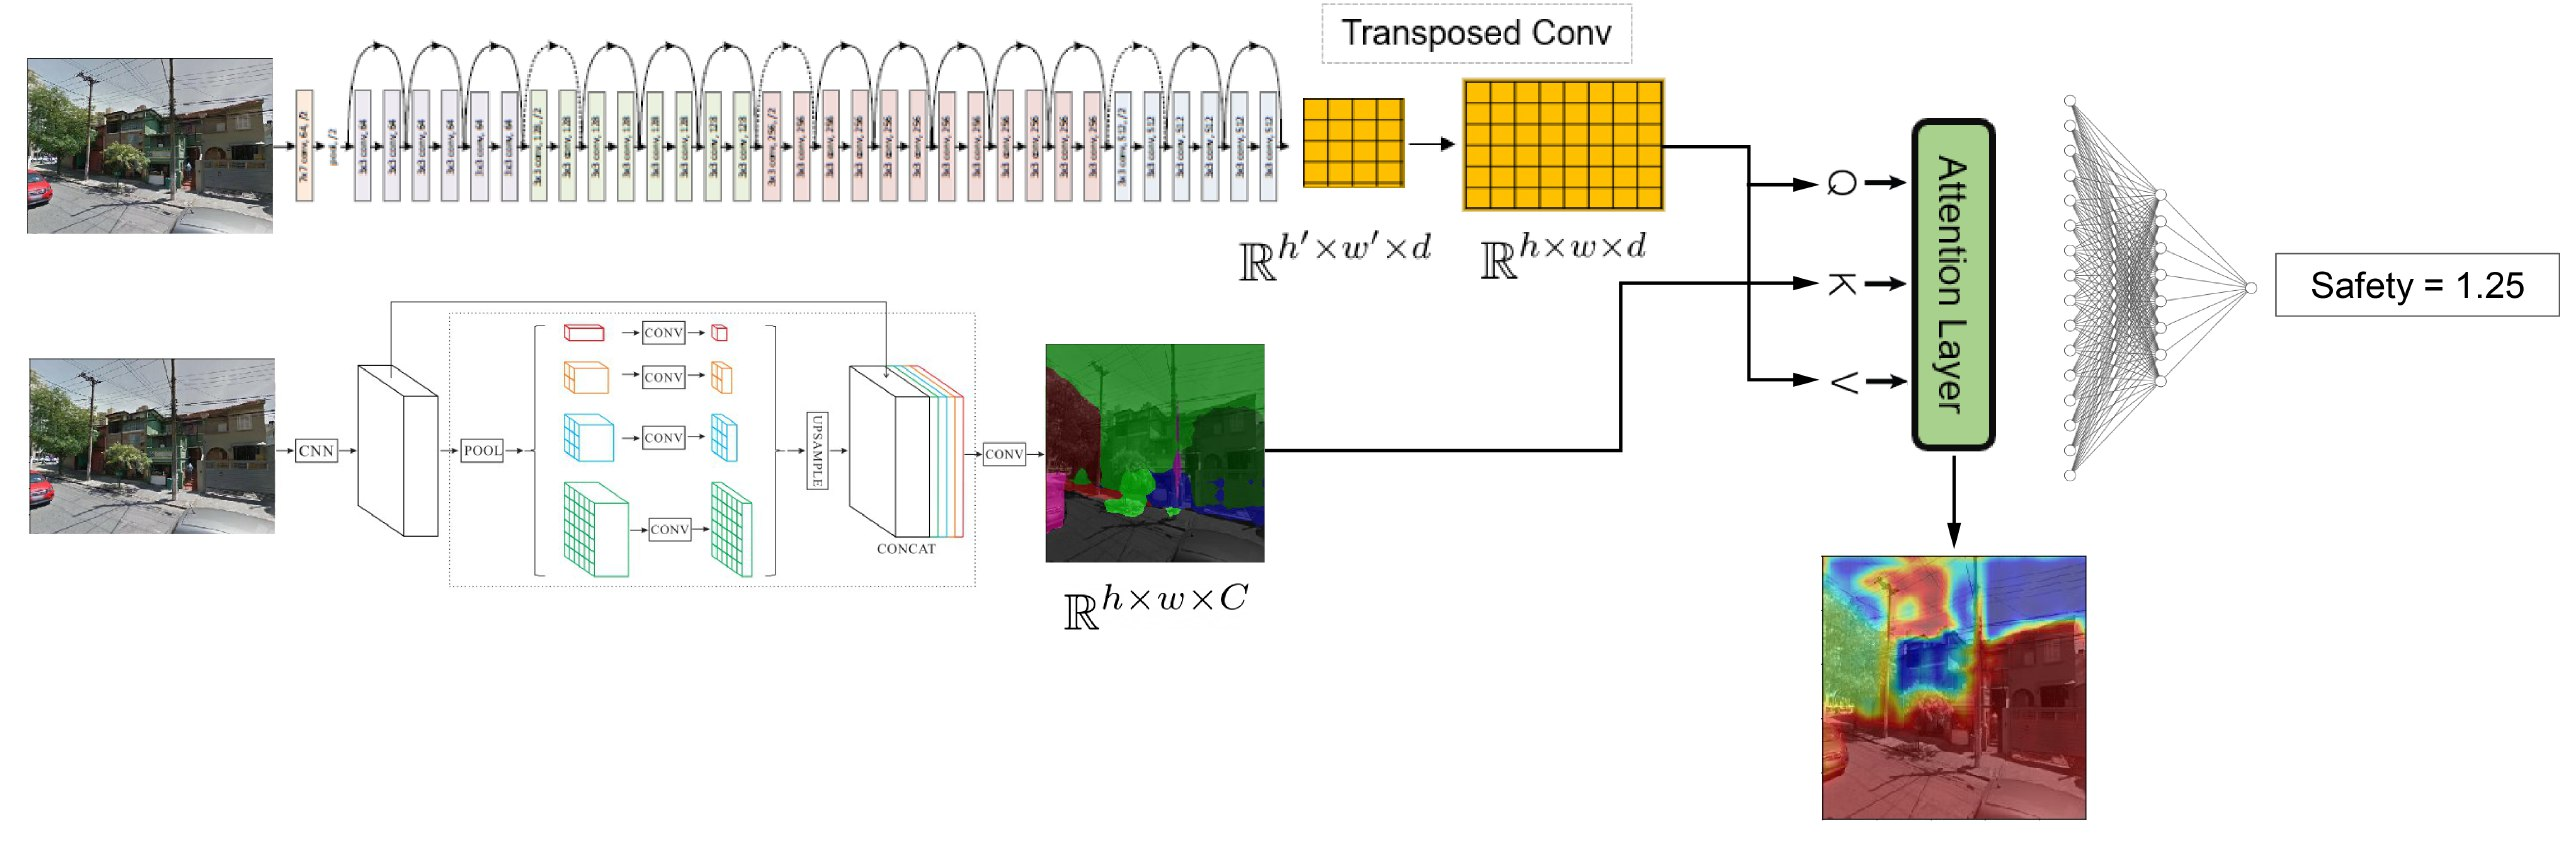
\includegraphics[width=1\textwidth]{./figures/segattn.png}
	\caption[Segmentation as key network]{Segmentation as key network.}
	\label{fig:segrank_1}
	\end{center}
\end{figure}

\section{Additional components}
\label{sec:adds}
\subsection{Loss function} \label{section:loss}
The loss function for this task must account for the pairwise structure of the dataset,
and should represent the cost of breaking restrictions given by Equations
\ref{eq:constraints} and \ref{eq:constraints_ties}. For \ref{eq:constraints} we use
a hinge loss similar to the one proposed by \citeA{hidalgo_placepulse}:

\begin{equation}
	L_r(x_1,x_1,y \mid \Theta) = \max(0, -y(f_\Theta(x_1) - f_\Theta(x_2)) + m_r)
	\label{eq:r_loss}
\end{equation}

Where $f_\Theta$ and $\Theta$  represent the network and its parameters respectively, and $m_r$
is an hyperparameter. This loss component makes it so that the model learns to assign a higher
score to the image winner of the vote. Based on the work by \citeA{doughty_loss} we also add a second component so that tied votes can
be used for training. According with equation \ref{eq:constraints_ties} we define:

\begin{equation}
	L_t(x_1,x_2 \mid \Theta) = \max(0, |f_\Theta(x_1) - f_\Theta(x_2)| - m_t)
	\label{eq:t_loss}
\end{equation}

Where $m_t$ is also an hyperparameter. Finally, the complete loss function is defined as:

\begin{equation}
	L(x_1,x_2,y \mid \Theta) =\left\{\begin{matrix}
		L_r(x_1,x_2,y)&\text{ if } y \in \{-1,1\} \\
		L_t(x_1,x_2)&\text{ if } y=0
	\end{matrix}\right.
\end{equation}

In practice we take the mean loss over the batch examples and we set $m_r=m_t=1$

\subsection{Semantic Dropout}
It's important to note that the semantic segmentation model trained on cityscapes,
presents an unavoidable drop in segmentation performance when applied on PlacePulse
due to domain shift. Errors in the segmentation can produce  significant problems
in the final perception quantification and can also cause confusing
attention heatmaps due to errors in the object edges.

In practice we identified a tendency for the models to have attention
weights highly biased towards specific segmentation classes, which is highly undesirable
both for explainability and model generalization.

We solve these problems by implementing what we call Semantic Dropout, similar to traditional Dropout \cite{srivastava_dropout},
but instead of dropping a single neuron with probability $p$, Semantic Dropout sets the
probabilities of an entire segmentation class to 0, inducing artificial errors
during training and preventing the network from becoming too sensitive to
segmentation errors while also reducing the bias in attention weights.
This effect can be seen on Figure \ref{fig:dropout}, which shows how the attention weights are less biased towards one class and therefore
less affected by the errors in segmentation.
Mathematically
this technique is equivalent to the spatial dropout proposed in \citeA{tompson_efficient},
but applied to segmentation probabilities instead to convolutional kernels.


\begin{figure}[!htb]
	\minipage{0.25\textwidth}
		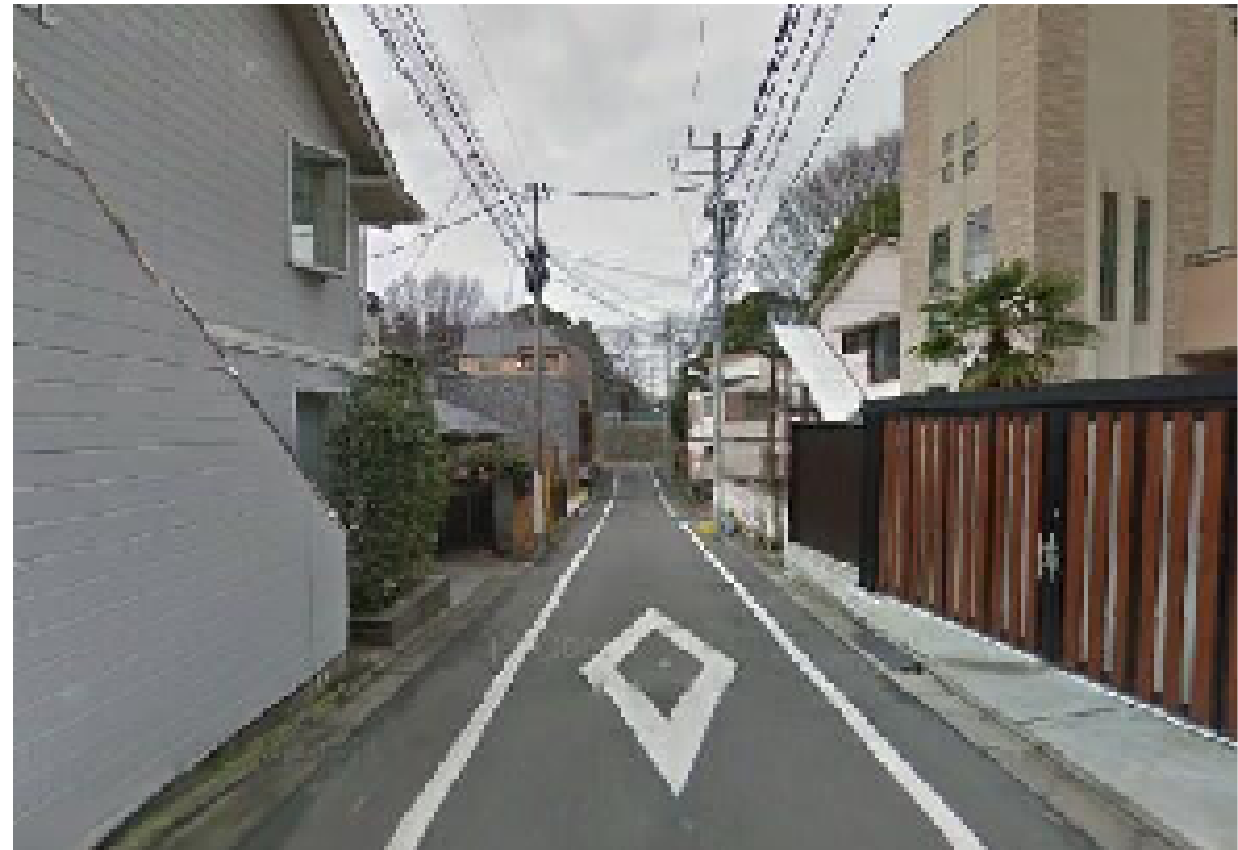
\includegraphics[width=\linewidth]{figures/original_sample.png}
	\endminipage\hfill
	\minipage{0.18\textwidth}
		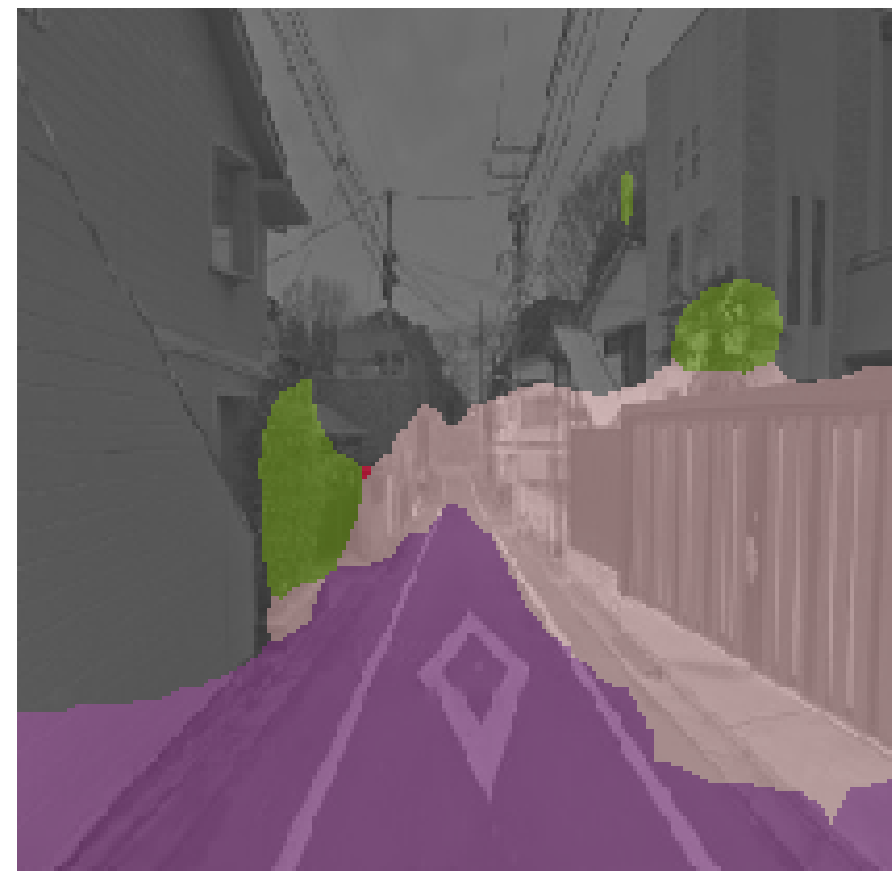
\includegraphics[height=\linewidth]{figures/segmentation_sample.png}
	\endminipage\hfill
	\minipage{0.26\textwidth}
		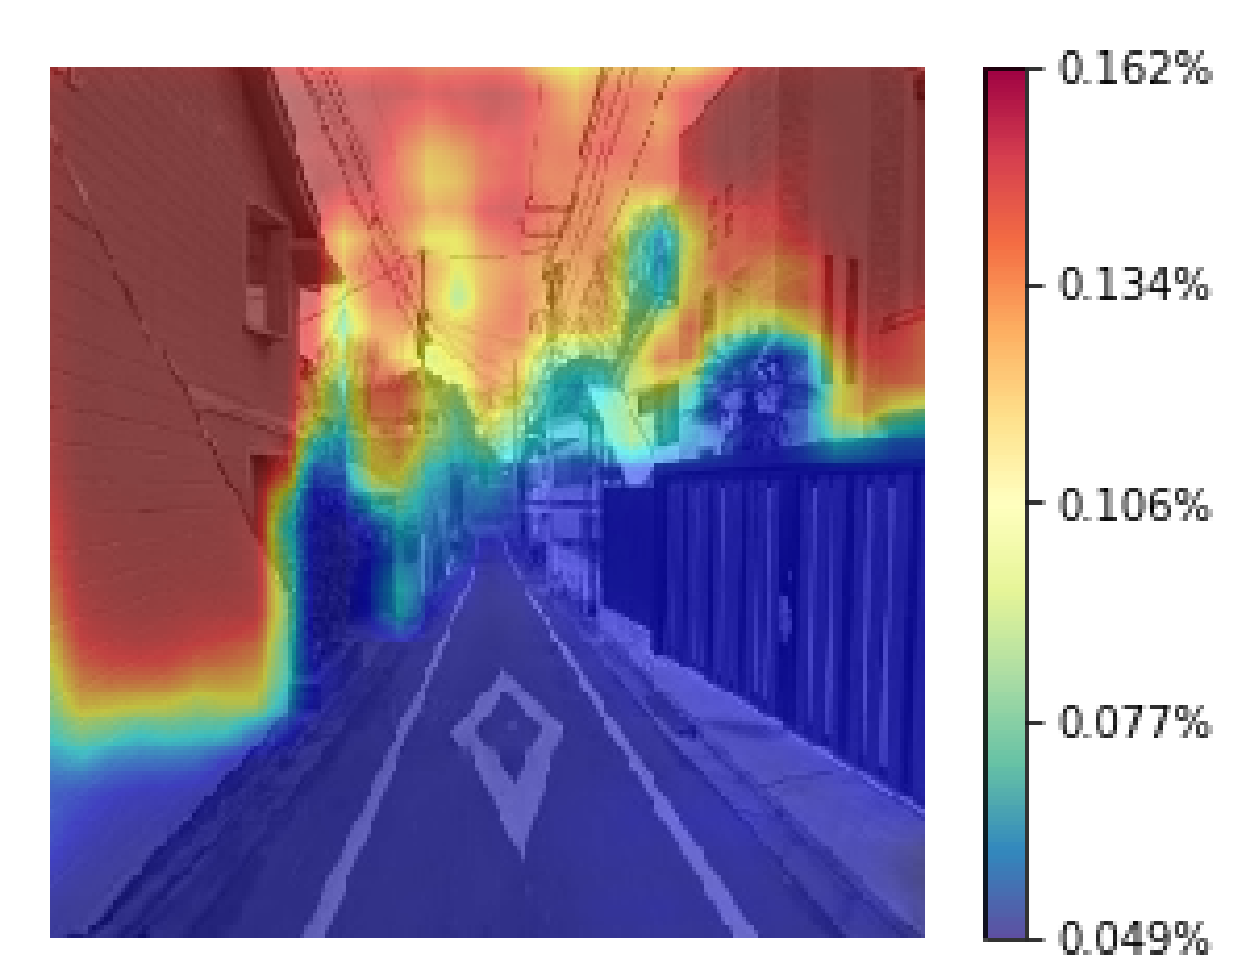
\includegraphics[width=\linewidth]{figures/segrank_sample.png}
	\endminipage\hfill
	\minipage{0.25\textwidth}
		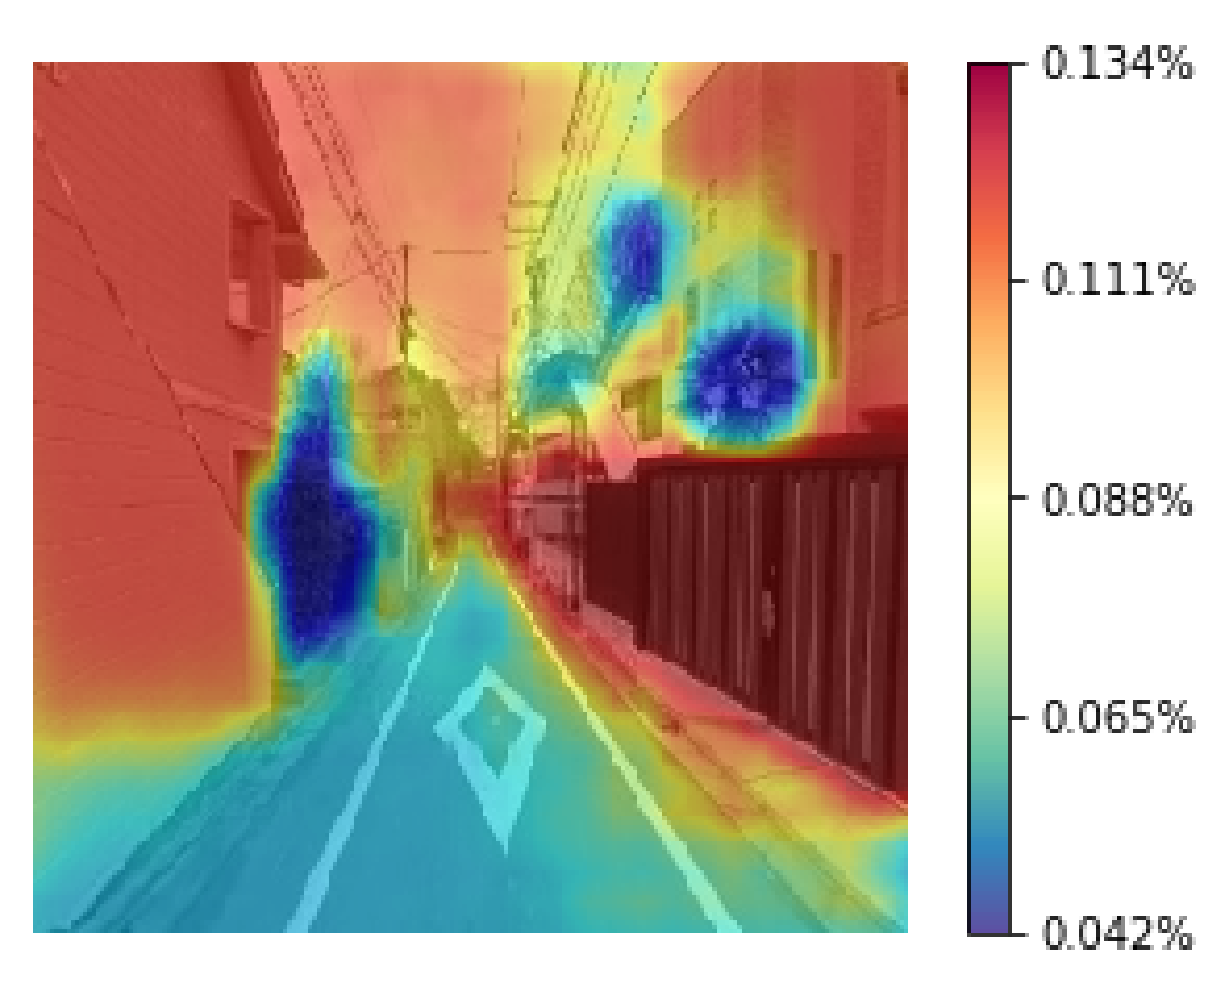
\includegraphics[width=\linewidth]{figures/segattn_sample.png}
	\endminipage
	\caption[Effect of Semantic Dropout]{
		Effect of Semantic Dropout. From left to right: original image, semantic segmentation
		and the outputs of the self attention model trained, without and with semantic dropout.
	}
	\label{fig:dropout}
\end{figure}

\section{Baselines}
\label{sec:baselines}
With the purpose of making and ablation study, we also train two baseline models
based on the architecture proposed by \citeA{hidalgo_placepulse}, designed for
measuring the effect of the segmentation and attention mechanisms in both performance
and explainability of the models. We base these models on the ResNet50 CNN \cite{he_resnet},
as is the defacto approach for computer vision problems. We abstain from using larger
versions of ResNet due to significant overfitting issues.

\subsection{ResNet50 + MLP}
The first baseline consists of a standard finetuned ResNet50 with a two layer MLP. This
model doesn't provide any sort of out of the box explainability and therefore is useful
to measure how segmentation affects performance.
Unlike its segmentation based sibling, dropout and L2 regularization are necessary for training
this model, due to the significantly larger amount of trainable parameters that come from finetuning the CNN.

\subsection{ResNet50 + Self Attention layer + MLP}

A baseline on explainability is also important, since improving it is the key contribution
of this work. For that we use a similar architecture to attention-based explainability
models from the literature \cite{zhang_interpretable, cordonnier_relationship, bello_attention}, consisting on
combining a finetuned CNN with self attention layers.

We take the output of ResNet50's \textit{conv\_5c} layers and give it to the attention layer
defined in Section \ref{section:self-attn} and then to a two layer MLP for calculation of the final score.

\begin{figure}[ht]
	\begin{center}
	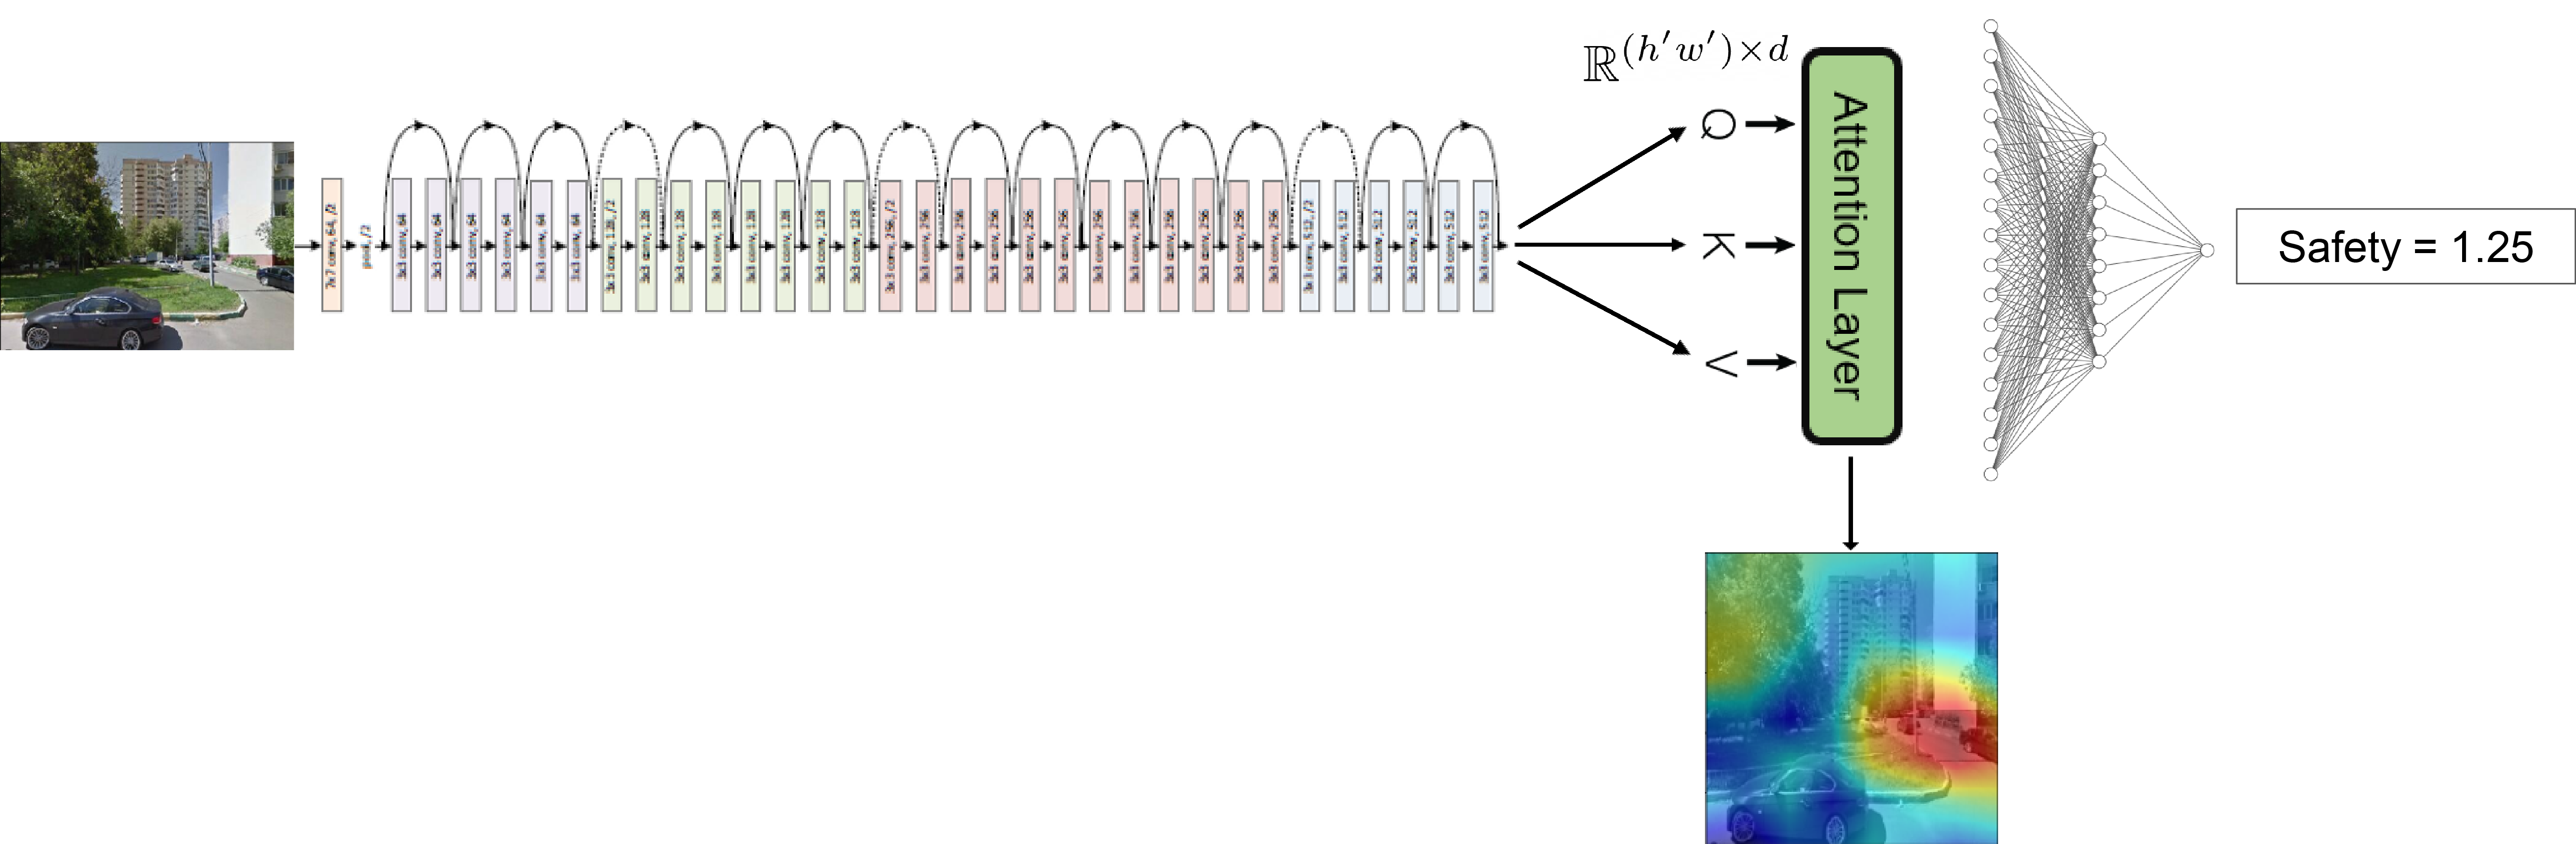
\includegraphics[width=1\textwidth]{./figures/attn_baseline.png}
	\caption[ResNet + SelfAttention]{ResNet and self attention network. ResNet diagram extracted from \citeA{he_resnet}.}
	\label{fig:attn_resnet}
	\end{center}
\end{figure}